% !TEX root = ../../thesis.tex

\chapter{Optimising Building Net Energy Demand with Dynamic BIPV shading}
\label{ch:asfSimulation}

\graphicspath{{chapters/ch2asfSimulation//Images/}}

\begin{chapterabstract}
TThe utilisation of a dynamic photovoltaic system for adaptive shading can improve building energy performance by controlling solar heat gains and natural lighting, while simultaneously generating electricity on site. This chapter firstly presents an integrated simulation framework to couple photovoltaic electricity generation to building energy savings through adaptive shading. A high-resolution radiance and photovoltaic model calculates the photovoltaic electricity yield while taking into account partial shading between modules. The remaining solar irradiation that penetrates the window is used in a resistance-capacitance building thermal model. A simulation of all possible dynamic configurations is conducted for each hourly time step, of which the most energy efficient configuration is chosen. We then utilise this framework to determine the optimal orientation of the photovoltaic panels to maximise the electricity generation while minimising the building's heating, lighting and cooling demand.  An existing adaptive photovoltaic facade was used as a case study for evaluation. Our results report a 20\% - 80\% net energy saving compared to an equivalent static photovoltaic shading system depending on the efficiency of the heating and cooling system. In some cases the Adaptive Solar Facade can almost compensate for the entire energy demand of the office space behind it. The control of photovoltaic production on the facade, simultaneously with the building energy demand, opens up new methods of building management as the facade can control both the production and consumption of electricity.
\end{chapterabstract}

\blfootnote{Jayathissa, P., Luzzatto, M., Schmidl, J., Hofer, J., Nagy, Z. \& Schlueter, A. Optimising Building Net Energy Demand with Dynamic BIPV shading. Applied Energy (2017)}

\newpage

\section{Introduction}
\label{ch:introduction2}
% !TEX root = B99_main.tex


Buildings are a critical element in our modern society and accommodate a variety of needs and functions. Unfortunately the energy consumed by buildings accounts for 32\% of global final energy consumption and 19\% of energy-related greenhouse gas emissions \cite{IPCC}. The existing building stock, therefore, offers a great potential for CO$_2$ mitigation of up to 50\% - 90\% using existing technologies \cite{IPCC}. Of these proposed technologies, building integrated photovoltaics (BIPV) have been recognised as a viable path to supply the energy needs of a building \cite{defaix2012technical,raugei2009life}. \\


Developments in efficiency and costs of thin-film BIPV technologies have brought new design possibilities \cite{NREL, kushiya2014cis, kaelin2004low,jelle2012building}. Their lightweight and flexible nature allows for easier and more aesthetically pleasing integration into the building envelope. Furthermore, from a life-cycle perspective as evaluated in Chapter \ref{ch:asfLCA}, there are attractive returns on embodied energy \cite{perez2012faccade,jayathissa2016life}. One such example is the application of thin film PV on glazed surfaces to create a semi transparent BIPV system \cite{li2009energy,peng2016numerical,vats2012energy}. Such systems not only generate electricity, but also influence the thermo-optic properties of a building, which in Los Angeles can reduce the HVAC energy demand by 30\% \cite{chae2014building}. However, when used in colder climates, the reduction of solar heat gains results in a net HVAC loss \cite{chae2014building}.

Dynamic building envelopes can mitigate this loss by actively controlling direct and indirect radiation into the building, while still responding to the occupant's desires \cite{loonen2013climate}. As seen in Figure \ref{fig:ASFschematic2} this mediation of solar radiation has the potential of improving daylight distribution, while simultaneously reducing heating and cooling demands \cite{nagy2016adaptive}. Using thin film solar panels as the shading element also allows for the simultaneous production of photovoltaic electricity. \\

%In addition, less power is required to actuate them, thus facilitating the development of dynamic envelope elements \cite{nagy2016adaptive, rossi2012adaptive}. \\

%Interestingly, the mechanics that actuate dynamic envelopes couples seamlessly with the mechanics required for facade integrated PV solar tracking. 

Previous research in this field can be divided into two categories: the integration of building energy performance simulation with shading, and the effects of BIPV on building energy performance. 

With respect to the first category, the effects of external shading on building energy performance have been widely studied \cite{bellia2014overview}. Palmero-Marrero et al. analyses the effects of external louvres using TRNSYS \cite{palmero2010effect}. The chapter shows that significant energy savings for space cooling is possible in hot climates, however in cities like London, the increase in the heating demand results in a net energetic loss. Nielsen et al. quantified the performance of dynamic solar shading systems using both building thermal and daylight simulations with a case study in Denmark \cite{nielsen2011quantifying}. The results show that a dynamic shading system is the best design alternative as it has an improvement in daylighting performance over fixed shading systems.\ 

Previous BIPV research analyses electricity production and building energy demand for static BIPV shading systems. Freitas et al. analyses different configurations of BIPV systems and shows that a tilted louvre configuration generates 20\% - 40\% more electricity than a flat vertical layout \cite{freitas2015maximizing}. Sun et al. analyses a static tilted photovoltaic system mounted over windows and reports a 51.6\% reduction in cooling demand \cite{sun2012optimum}. Mandalaki et al. expands this analysis to 13 different types of shading devices with integrated PV \cite{mandalaki2012assessment}. Hu et al. combines PV production with building energy performance in an analysis of Trombe wall systems and finds that a Trombe wall with PV venetian blinds has a 45\% energy saving when compared to classic PV Trombe wall systems \cite{hu2017comparative}. Optimising the panel angles for PV production however are not always advantageous. Chatzipanagi et al. demonstrated that an inclination of 30$^{\circ}$ of integrated crystaline modules results in very high operating temperatures, thus penalising the system \cite{chatzipanagi2016bipv}. It is therefore important to also include thermal effects in BIPV analysis. \\

%\added[id=pj, remark=``This version was created based on Zoltans comments on the previous iteration'']{V1: We have previously combined the two aforementioned categories to evaluate the annual performance of a dynamic photovoltaic shading system and its impact on the building energy demand \cite{jayathissa2016PVSEC}. The methodology was sufficient to attain an understanding of how such a system functions, however it used simplifications that ignored time dependant characteristics of the building, such as thermal capacitance. This chapter expands on this previous research in two parts. Firstly, by running hourly simulations that combine the electricity production of the dynamic shading system with the building energy demand. Secondly, by proposing a novel adaptive control strategy where the results of each hourly simulation are used to determine the orientation of the PV panels. By doing so, we can not only evaluate the hourly performance of an adaptive photovoltaic shading system, but can also use the same framework to control the physical system.}\\

This chapter expands on this previous research in two parts. Firstly, by combining the two aforementioned categories to evaluate a dynamic photovoltaic shading system and its interaction with the building energy demand. Secondly, by proposing a novel adaptive control strategy where the results of the simulation are used to determine the orientation of the PV panels. We have previously modelled the energy performance of dynamic BIPV shading systems \cite{jayathissa2016PVSEC}. The methodology was sufficient to attain an understanding of how such a system functions, however it used simplifications that ignored time-dependent characteristics of the building, such as thermal capacitance. \\


The contribution of this chapter is a simulation framework that overcomes these simplifications, in order to evaluate the energetic performance of adaptive photovoltaic envelopes with respect to PV electricity production and building energy demand. The framework is applied in the context of the Adaptive Solar Facade (ASF) project, shown in Figure \ref{fig:HoNR2} \cite{nagy2016adaptive}. The ASF is a lightweight PV shading system composed of dynamically actuated copper indium gallium selenide (CIGS) panels. CIGS panels from Flisom were chosen due to their light-weight nature, high efficiency, and monolithic interconnection, however in principle any light-weight PV material can be used \cite{feurer2016progress}. Each panel can independently rotate in two degrees of freedom, through the use of a soft pneumatic actuator \cite{svetozarevic2016soro}. This freedom enables local variations of the facade when reacting to internal and external factors.  For more information on the technology, please refer to the publication by Nagy et al. \cite{nagy2016adaptive}.\\





The remainder of the chapter is organised as follows. The next section describes the simulation methodology including the case study used in the analysis. In Section \ref{ch:results2} the results of the case study are presented which describes the adaptive response of the ASF to variations in the external and internal environment. Finally, Section \ref{ch:conclusion2} concludes the chapter.




\begin{figure}
\begin{center}
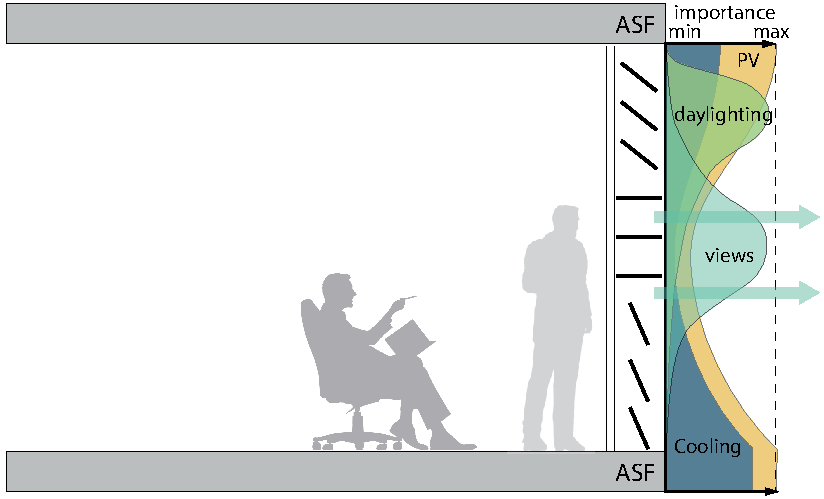
\includegraphics[width=8cm, trim= 0cm 0cm 0cm 0cm,clip]{facadeFunctionsnew.pdf}
\caption{The facade acting as a mediator between the interior and exterior environment, while fulfilling various functions \cite{nagy2016adaptive}}
\label{fig:ASFschematic2}
\end{center}
\end{figure}

\begin{figure}
\begin{center}
\includegraphics[width=8cm, trim= 0cm 0cm 0cm 0cm,clip]{honr.jpg}
\caption{An example of an ASF constructed at the House of Natural Resources \cite{nagy2016adaptive}}
\label{fig:HoNR2}
\end{center}
\end{figure}






\section{Methodology}
\label{ch:method2}
% !TEX root = B99_main.tex



The proposed framework is shown schematically in Figure \ref{fig:workflow2}. In brief, it consists of five stages. First, the radiation on the PV panels and office window is calculated for a single configuration of the ASF. The radiation results on the PV panels are then used to calculate the electricity generation. The radiation results on the window are imported into a building thermal model, and a separate lighting model. Finally, an exhaustive search of all possible configurations is performed to determine the optimal configuration for maximum energetic performance. The framework along with installation guides are publicly available for download \cite{ASFGitHub,RCGitHub} . The following subsections detail these five stages.



\begin{figure}
\begin{center}
\begin{tikzpicture}[node distance = 2cm, auto]
    % Place nodes
    \node [block] (m1) {Initialisation};
    \node [block, below of=m1, node distance=4cm] (init) {Radiation Analysis};
    \node [block, below left of=init, node distance=4cm] (circuit) {PV Circuit Simulation};
    \node [block, below of=init, node distance=2.83cm] (rc) {RC Model};
    \node [block, below right of=init, node distance=4cm] (light) {Daylighting Model};
    \node [block, below right of=circuit, node distance=4cm] (optimise) {Optimisation};
    \node [text width = 5cm, below of=optimise] (result) {Optimal Configuration and Energy Performance for $t_k$};

    % Draw edges
    \path [line] (m1) -- node[ text width=3.2cm, auto, xshift=0em] {-Facade Geometry \\ -Weather Data \\ -Building Data \\ -Orientation}(init);
    \path [line] (optimise) -- (result);
    \path [line] (init) -- (circuit);
    \path [line] (init) -- (rc);
    \path [line] (init) -- (light);
    \path [line] (circuit) |- node[near start, text width=2cm, left, yshift=0.7em] {Electricity \\ Supply} (optimise);
    \path [line] (rc) -- node[anchor=center, text width=3cm, right, xshift=0em] {Heating/ \\ Cooling \\ Demand} (optimise);
    \path [line] (light) |- node[near start, text width=3cm, right, yshift=0.8em] {Lighting \\ Demand} (optimise);
    \path [line, dashed] (result) -- ++(6cm,+0cm) |- node[near end, yshift=1.5em] {Building Data from $t_{k-1}$} (init);

\end{tikzpicture}
\caption{Simulation workflow}
\label{fig:workflow2}
\end{center}
\end{figure}



\subsection{Radiation Analysis}
\label{ch:rad}
A solar radiation simulation is run within the Rhino/Grasshopper environment \cite{grasshopper} with the Ladybug plugin \cite{roudsari2013ladybug},  that uses Radiance \cite{ward1994radiance} to determine the incident insolation on the solar facade. The solar radiation analysis implemented in Ladybug is based on the cumulative sky approach \cite{robinson2004irradiation} using the Perez All-Weather sky model and weather files with hourly resolution \cite{perez1993all}. In this analysis, the sky is divided using the Tregenza scheme \cite{tregenza1987subdivision}. The approach enables us to calculate solar irradiance on the modules, and the glazed surface behind the facade. Self shading of the PV modules is inevitable as the gap between modules is only 100mm. The modules were therefore divided with a gird size of 25mm to include the effect of mutual shading as seen in Figure \ref{fig:radiation2}.
  

\subsection{PV Circuit Simulation}

The radiation results are coupled using Python to an electrical circuit simulation of monolithically interconnected, thin-film CIGS PV modules with sub-cell level representation \cite{hofer2016parametric,python}. This model uses the standard equivalent circuit model to calculate sub-cell current-voltage curves with a single diode, one series resistor, and one shunt resistor \cite{mermoud2010}. By doing so, the electrical losses through module self shading, as described in Section \ref{ch:rad}, can be taken into account. In addition to the irradiation dependency, the PV simulation includes temperature dependency. A linear relation between PV cell operating temperature and incident solar irradiance is assumed \cite{skoplaki2009operating}. Infra-red thermal imaging at different irradiance levels was used to infer the correlation factor. Electro-thermal effects and the influence of wind are neglected in the model. For more information, please refer to the publication by Hofer et al. \cite{hofer2016parametric}.


\begin{figure}
\begin{center}
\includegraphics[width=\columnwidth, trim= 0cm 0cm 0cm 0cm,clip]{radiationAnalysis.png}
\caption{A simulation result showing module and window insolation from 11:00 - 12:00 on the 16 June for a Zurich weather file and a specific module orientation.}
\label{fig:radiation2}
\end{center}
\end{figure}


\subsection{RC Model for Building Energy Demand}

This subsection describes the formulation of a physics-based model to simulate the thermal behaviour of the building using a resistor-capacitor (RC) model. This is based on an electrical analogy corresponding to the equivalent thermal physics \cite{bacher2011identifying, sonderegger2010diagnostic, madsen1995estimation}. The model, shown in Figure \ref{fig:RC_Model}, consists of one internal thermal capacitance, and five thermal resistances. This is also known as a 5R1C model and is based on the ISO 13790 standard \cite{de2008iso}. It is briefly reviewed here for completeness.

\begin{figure}
\begin{center}
    \begin{circuitikz}
      \draw (0,0)
      node[label={left:$T_e$}] {}
      to[short,*-] (1,0)
      to[short] (1,1)
      to[european resistor=$H_w$] (3,1); % The resistor

      \draw(1,0)
      to[short] (1,-1)
      to[european resistor=$H_{em}$] (3,-1)
      node[label={10:$T_m$}] {}
      to[european resistor,l_=$H_{ms}$] (3,1)
      node[label={10:$T_s$}] {}
      to[european resistor,l_=$H_{is}$] (3,3)
      node[label={10:$T_{air}$}] {}
      to[european resistor,l_=$H_{ve}$] (1,3)
      to[short,-*] (0,3)
      node[label={left:$T_{sup}$}] {};

      \draw(3,-1)
      to[short,*-] (5,-1)
      to[short,-*] (5,1)
      to[short,-*] (3,1);

      \draw(5,1)
      to[short] (5,3)
      to[short,-*] (3,3)
      to[european current source,l_=$\phi_{HC}$] (3,5);

      \draw(5,1)
      to[european current source,l_=$\phi_{sol}+\phi_{int}$] (7,1);

      \draw(3,-1)
      to[C=$C_m$] (3,-2)
      node[ground]{};


    \end{circuitikz}
    \caption{A 5R1C Model of the single zone office space}
\label{fig:RC_Model}
\end{center}
\end{figure}


The only surface in contact with the external environment is the south facing glazed surface. All other surfaces of the room are in contact with other thermal zones of the building that are assume to hold the same room temperature. They can therefore be modelled as adiabatic surfaces. Denoting by $T_m$, the temperature of the thermal mass in the room, the differential equation for the circuit in Figure \ref{fig:RC_Model} is given by 

%Equation \ref{eq:derrive} details the equation related to the circuit in Figure \ref{fig:RC_Model} where $T_m$ is the temperature of the room mass, and $C_m$ is the thermal capacitance of the room. 


\begin{equation} 
\label{eq:derrive}
     C_m {\frac{dT_m}{dt}} + T_m(H_{tr3}+H_{em})  = \phi_{mtot}
\end{equation}

The value $\phi_{mtot}$ represents an equivalent thermal heat flux based on the solar heat gains, internal heat gains, external air temperature and the thermal conductances of the building elements. For this analysis variations of air convection caused by the solar facade are ignored. For more information on this model, refer to the Appendix, or the source code on GitHub \cite{RCGitHub}. \\

% \begin{equation} 
% \label{eq:heatflow}
%       \phi_{mtot}= \phi_m + H_eT_e + \frac{H_{tr3}}{H_{tr2}}\Big(\phi_{st} + H_wT_e + H_{tr1}T_{sup} + \frac{H_{tr1}}{H_{ve}}(\phi_{HC} + \phi_{io})\Big)
% \end{equation}



%where $C_m$ is the thermal capacitance of the room, $T_e$ is the external air, $T_{sup}$ is the conditioned air supply. The solar heat gains $\phi_{sol}$, and internal heat gains $\phi_{int}$ are represented by three equivalent heat fluxes $\phi_{io}$, $\phi_{st}$ and $\phi_m$ which correspond to a heat exchange to the air $T_{air}$, internal room surface $T_s$, and thermal mass $T_m$ respectively. The heating and cooling heat flux is represented by $\phi_{HC}$. The five thermal conductances $H$ are represented by three equivalent conductances $H_{tr1}$, $H_{tr2}$, $H_{tr3}$. For more information on the model, refer to the Appendix. 

Equation \ref{eq:derrive} is discretised using the Crank-Nicolson method so it can be solved numerically as,

%Applying the Crank-Nicolson method \cite{crank1947practical} to Equation \ref{eq:derrive} gives us the discrete differential equation described in Equation \ref{eq:derivation}. The subscripts $k$ and $k+1$ refer to the timesteps of length $\Delta t$. 

\begin{equation} 
\label{eq:derivation}
      T_{m_{k+1}}={\frac{\phi_{mtot}+T_{m_k}\Big(\frac{C_m}{\Delta t} - 0.5(H_{tr3}+H_{em})\Big)}{\frac{C_m}{\Delta t} + 0.5(H_{tr3}+H_{em})}}
\end{equation}

where the subscripts $k$ and $k+1$ refer to the time-steps of length $\Delta t$ \cite{crank1947practical}.\\

The heating or cooling demand for each time step is determined to ensure that the temperature $T_{m_{k+1}}$ is within the set thermal set points for occupant comfort. An unrestricted heating or cooling system is assumed. This means that the heating or cooling supply will always meet the calculated demand. The thermal demand is converted to electrical energy based on an average coefficient of performance (COP) of the heating or cooling system. 

\subsection{Lighting Model}
Lighting control is based on the average luminance of the room. The luminance that passes through the solar facade, to the window, is calculated in the radiation analysis in Section \ref{ch:rad}. Using the total flux method \cite{szokolay1980handbook}, the total luminance per floor area is calculated by 

\begin{equation} 
\label{eq:lighting}
      \varphi_{flux}={\frac{E_w G M U}{A_{floor}}}
\end{equation}

where $E_w$ is the incident illuminance on the window, $G$ is the solar transmittance of the window, $M$ is the maintenance factor which takes surface dust into account, and $U$ is an empirical utilisation factor based on the room dimensions and ceiling profile. If the room luminosity is less than the set threshold for comfortable lighting, and there are occupants in the room, the lights are switched on to their maximum power. When compared against a more complex Radiance model with ambient bounces there was only a 5\% divergence in results. The total flux method was therefore chosen due to its computational speed. This method however, is only applicable for small spaces. The evaluation of a hall, or an open plan working space would require a ray tracing analysis with multiple bounces. The electrical wiring and pneumatics of the ASF are encased within a reflective double curved stainless steel pipe structure that takes 6\% of the projected area. The influence of this structure can therefore be assumed to be negligible. 

\subsection{Exhaustive Search Optimisation}

At each time step the combination that minimises the net building energy demand, i.e. the difference of building energy demand for heating, cooling, lighting against BIPV electricity generation, is found using an exhaustive search of all possible configurations. Transient elements of the results, such as the temperature of the room, and thermal control settings are then stored for the next time step. It is also possible to run this optimisation to minimise individual objectives, such as heating alone.

% \begin{figure}
% \begin{center}
% 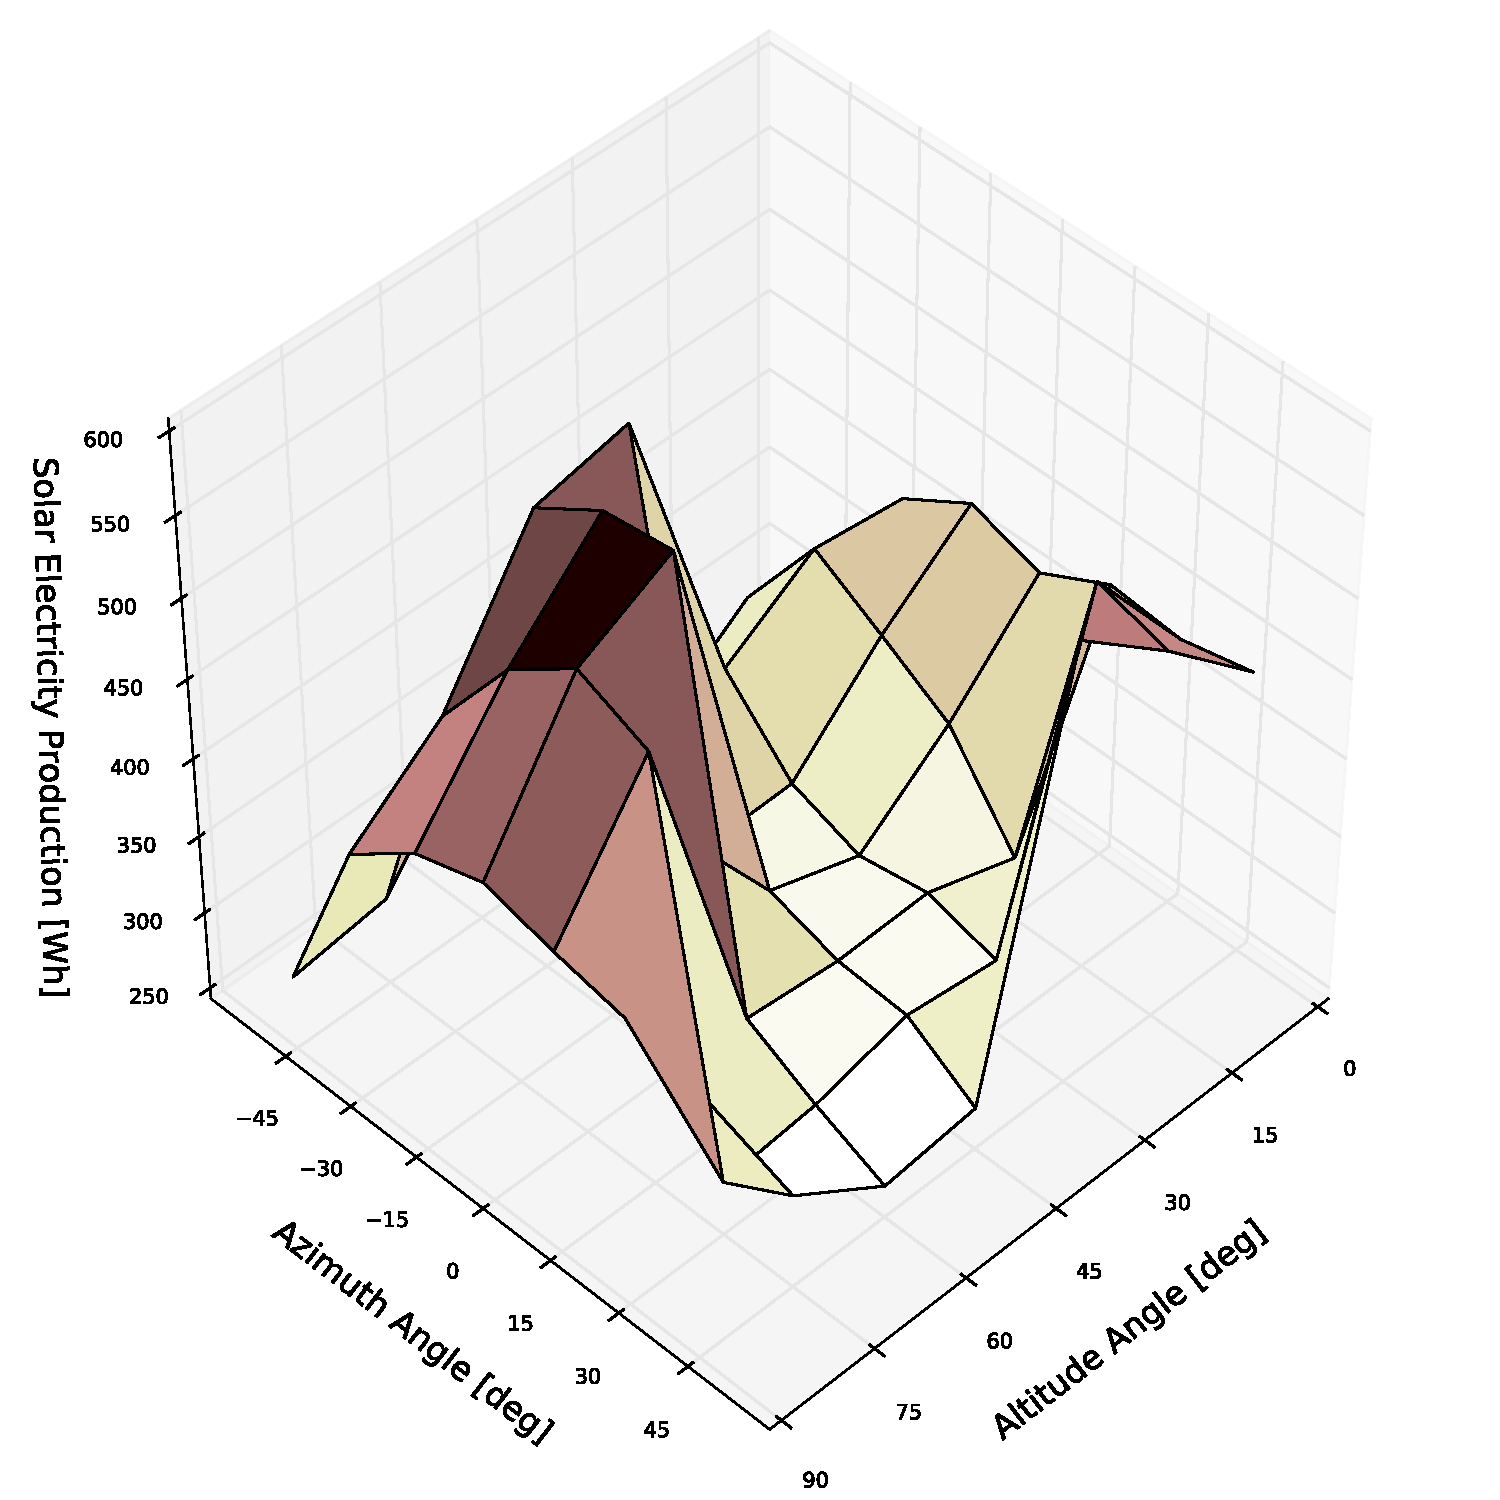
\includegraphics[width=\columnwidth, trim= 0cm 0cm 0cm 0cm,clip]{3DAnglePlot.pdf}
% \caption{ }
% \label{fig:optimsationAngles}
% \end{center}
% \end{figure}


\subsection{Case Study}

The ASF, shown in Figure \ref{fig:HoNR2}, was constructed on the House of Natural Resources at the ETH Zurich \cite{nagy2016adaptive}. This system is used as a case study for the framework. The solar facade consists of 400mm CIGS square panels that can rotate in two degrees of freedom via a soft pneumatic actuator \cite{svetozarevic2016soro}. Each panel can be independently actuated with a continuous range of actuation. However, for simplicity, all panels are grouped into one cluster that moves in unison with discrete angles. On the horizontal axis, the panels can move from 0$^{\circ}$ (closed) to 90$^{\circ}$ (open) position in steps of 15$^{\circ}$. On the vertical axis, they can move from 45$^{\circ}$ to -45$^{\circ}$ in 15$^{\circ}$ steps. This results in 49 possible dynamic configurations of the facade system.

The studied building is a two person office which is 3.1m high, 4.9m wide, and 7m deep. Input data for the simulation is based on an energy plus weather file for the Zurich region \cite{remund1997meteonorm}. The weather data is recorded at an hourly resolution, and therefore the simulation is also run at hourly time-steps. A full set of input parameters for this case study is summarised in Table \ref{tab:AssumptionsOpp}.



\begin{table*}
\centering
\begin{tabular*}{\textwidth}{ll}
\hline
\textbf{Office Zone Settings} &                                        \\
Office Envelope               & Internal Walls: Adiabatic              \\
                              & Window: Double Glazed U=1.1 $W/m^2K$     \\
                              & External Wall: U=0.2 $W/m^2K$            \\
Daylighting Variables         & Glass Solar Transmittance: 0.68                          \\
                              & Maintenance Factor: 0.9                \\
                              & Utilisation Factor: 0.7               \\
Thermal Conductances          & $H_{ve}=39 W/K  $                      \\
                              & $H_{w}=14.9 W/K $                      \\
                              & $H_{em}=0.34 W/K$                      \\
                              & $H_{is}=491 W/K $                      \\
                              & $H_{ms}=780 W/K $                      \\
Thermal Set Points            & Heating: 22$^{\circ}$C                 \\
                              & Cooling: 26$^{\circ}$C                 \\
                              & Set-Back: 4$^{\circ}$C                 \\
Building System               & Lighting Load: 11.8 $W/m^2$             \\
                              & Lighting Control Threshold: 300 lx     \\
                              & COP Heating: 3                         \\
                              & COP Cooling: 3                         \\
Occupancy                     & Office Schedule  \cite{CEAToolbox}     \\
                              & Ventilation: 1.5 air changes per hour  \\
                              & Infiltration: 0.5 air changes per hour \\
                              & Human Heat Emission: 120$W$ per person                                       \\
\textbf{Location Assumptions} &                                        \\
Weather File                  & Zurich-Kloten, Switzerland 2013 \cite{remund1997meteonorm}       \\
Window Orientation                   & South                                  \\
\hline
\end{tabular*}
\caption{Summary of simulation parameters}
\label{tab:AssumptionsOpp}
\end{table*}







\section{Results}
\label{ch:results2}
% !TEX root = B99_main.tex

% \begin{figure}
% \begin{center}
% \includegraphics[width=8cm, trim= 0cm 0cm 0cm 0cm,clip]{radiationanalysis.png}
% \caption{Incident radiation on the PV panels. Light blue spots indicate areas of self-shading}
% \label{fig:radiationanalysis}
% \end{center}
% \end{figure}


In this section we show the results of the framework applied to the case study. Section \ref{ch:transient} details the daily performance, this is then expanded in Section \ref{ch:optimal} for results spanning one year. Section \ref{ch:comparison} then compares this performance with a static shading system, and a facade with no shading. For each evaluation the thermal energy demands have been converted to an electrical energy input based on the coefficient of performance of the heating or cooling system.

\subsection{Daily Energetic and Control Profiles of the ASF}
\label{ch:transient}
We run the optimisation for the net energy minimisation. The results, shown in Figure \ref{fig:transient}a detail the simulation run on a sunny day in winter. The dashed line details the optimum altitude angle from an open (90$^{\circ}$), to a closed (0$^{\circ}$) position, and the azimuth angles from a south-east facing (45$^{\circ}$) to a south-west facing (-45$^{\circ}$) direction. We can see that the the azimuth angles start at an east facing position, roughly around 30$^{\circ}$, and switches to a west facing position, around -30$^{\circ}$ in the afternoon. The building energy demand consists of heating (H) and lighting (L) loads in the morning and evening. We can see that between 10:00 to 15:00 the PV panels are capable of generating more electricity (PV) than the office requires. 

Figure \ref{fig:transient}b compares this simulation with a sunny day in summer. The main energetic difference is the presence of a cooling (C) load in the afternoon. The panels still move in the azimuth directions from east to west, however the panels in the altitude direction sit at a higher angle to catch the higher sun position. The patterns in the summer and winter cases are representative of a solar tracking model, however, in both cases it appears to be limited between $\pm$30$^{\circ}$. This is most likely due to high module self-shading at $\pm$45$^{\circ}$, resulting in a large decrease in the PV module efficiency. In winter, the altitude angle is relatively stagnant at 15$^{\circ}$. This angle is sufficient to maximise the PV electricity generation, while still allowing enough solar penetration into the room to keep the lighting and heating demands to a minimum. 

In comparison, Figure \ref{fig:transient}c, details an optimisation on the same winter day, purely to minimise the heating load. In this case, the PV electricity generation, lighting demand, and cooling demand are not taken into account. There are two observable differences in the choice of angles. Firstly, the angles in the altitude position are mostly in the open (90$^{\circ}$) position. Secondly, the azimuth angles follow an inverse solar tracking methodology, starting with west facing angles in the morning, and moving to east facing directions in the evening. Both effects maximise the solar penetration into the room and therefore minimise the heating demand (red line), at the expense of the PV electricity generation (gold line). A similar comparison was conducted for the summer case where a simulation was run purely to optimise the cooling load as seen in \ref{fig:transient}d. The optimum angles to minimise cooling are similar to the optimum angles to minimise net energy so there are only minor differences in the chosen angles.
%However, these minor differences increase the PV generation by 19.5\%, and decreases the lighting by 50\% with only a 5\% increase in the cooling load. This ultimately decreases the net energy consumption of the day from 1151 Wh to 132 Wh.

It is also interesting to note that a sunny day in winter produces 3.0kWh of electricity, while a sunny day in summer produces only slightly more at 3.8kWh in the net energy optimisation case. This is due to the variation in the sun position. The  low winter sun position combined with solar tracking means that the panels are often perpendicular to the direction of the solar radiation. In summer, on the other hand, there is a high sun position, resulting in module self-shading which decreases the efficiency of the PV panels. Over the full day, the PV electricity supply compensates for 62\% of the energy demand on this sunny winters day, and 270\% of the energy demand on a sunny summers day. 


% \begin{figure}
% \begin{center}
% \includegraphics[width=\textwidth, trim= 0cm 0cm 0cm 0cm,clip]{HourlyPlot_WinterNew.pdf}
% \caption{Net energy optimisation and adaptation of the ASF on a sunny day in winter. The solid lines detail the energy balance of heating (H), lighting (L), PV electricity production (PV) and net energy (E) in Watt-hours. The dashed lines detail the panel position in the altitude angle from open (90$^{\circ}$), to a closed (0$^{\circ}$) position, and in the azimuth direction from a south-east facing (45$^{\circ}$) to a south-west facing (-45$^{\circ}$) direction. Only daylight hours are shown for the angle optimisation}
% \label{fig:transientWinter}
% \end{center}
% \end{figure}

\begin{figure}
\begin{center}
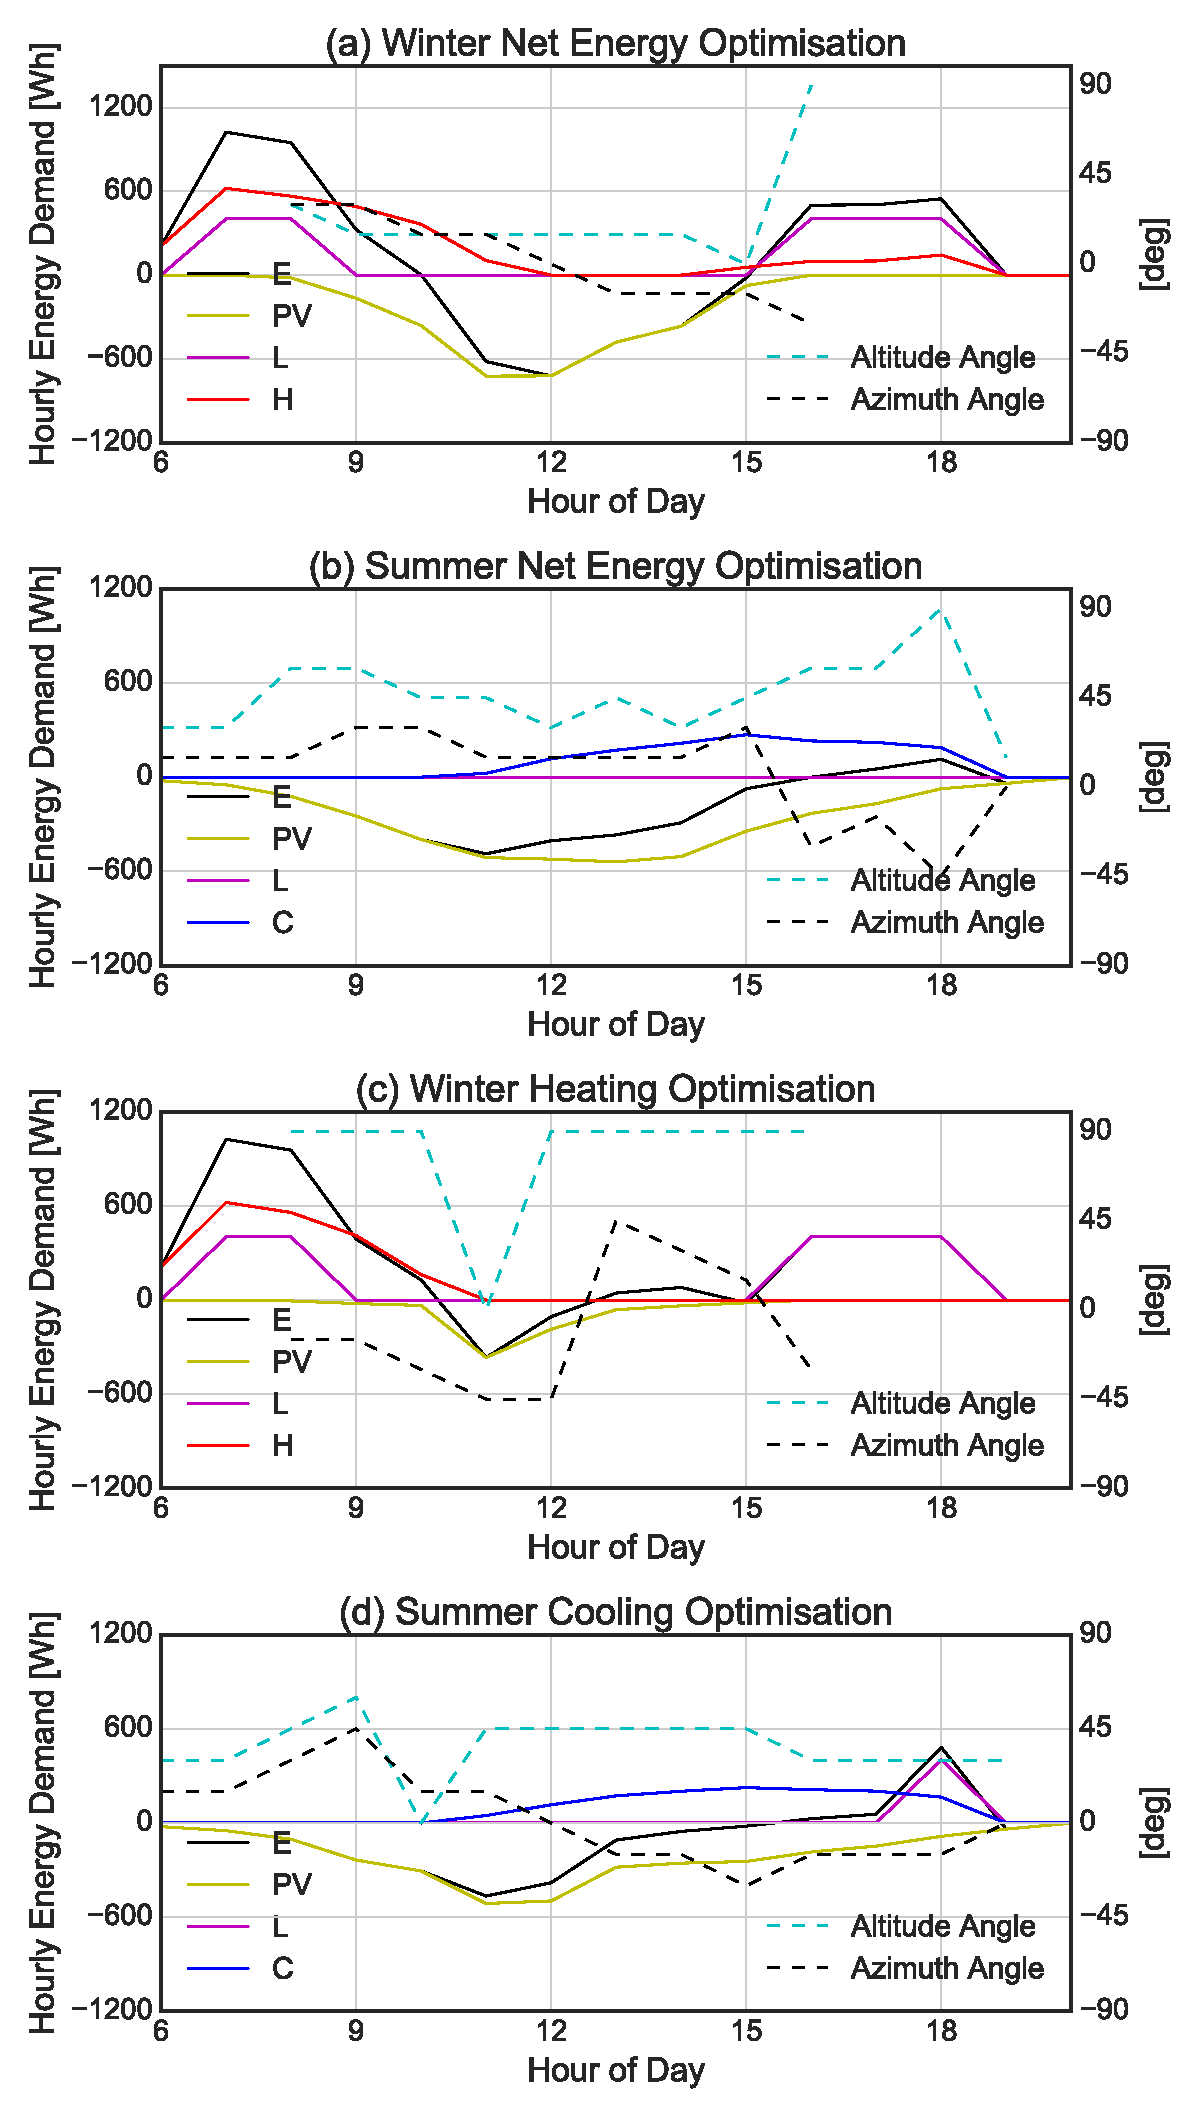
\includegraphics[width=0.65\textwidth,, trim= 0cm 0cm 0cm 0cm,clip]{HourlyPlotNew3.pdf}
\caption{Net energy optimisation and adaptation of the ASF on a sunny day in winter (a) and summer (b). The solid lines detail the energy balance of heating (H), lighting (L), Cooling (C), PV electricity production (PV) and net energy (E) in Watt-hours. The dashed lines detail the panel position in the altitude angle from open (90$^{\circ}$), to a closed (0$^{\circ}$) position, and in the azimuth direction from a south-east facing (45$^{\circ}$) to a south-west facing (-45$^{\circ}$) direction. Only daylight hours are shown for the angle optimisation. In Figures (c) - (d) the optimisation is restricted to just the heating optimisation and cooling optimisation in winter and summer respectively.}
\label{fig:transient}
\end{center}
\end{figure}

\subsection{Optimum Annual Configurations}
\label{ch:optimal}

The optimal configurations of the ASF case study over a year can be visualised using heat-maps. Figure \ref{fig:monthly_altitude} and \ref{fig:monthly_azimuth} detail the optimal angle in the altitude and azimuth angles respectively. To accelerate the radiation analysis, the weather data for each month is averaged to acquire data for a typical day of that month. Figure \ref{fig:monthly_altitude}a-d detail optimisations of individual objectives. We can see how open configurations (light colours) are often chosen for the minimisation of the heating and lighting demands. Likewise, closed configurations (dark colours) are the preferred solutions to minimise the cooling demand during the summer months. Interestingly, this trend appears to inverse during the summer months at midday. The high sun position favours open positions to maximise shading thus minimising cooling in summer. Likewise closed positions with maximum tilt in the azimuth angle maximise solar penetration, and thus minimise heating. The grey coloured points indicate times where there is no sun and therefore the ASF has no influence on the results. 
%Black coloured points areas where there is the combination of the ASF has no impact on the energy load. For example, in summer, no heating is required, therefore there is no optimal angle combination to reduce this any further. 

%The PV optimisation, best seen in Figure \ref{fig:monthly_azimuth}(d), follows a path similar to a classic solar tracking model. The variation from a solar tracking model is due to the effects of self-shading. 

\begin{figure*}
\begin{center}
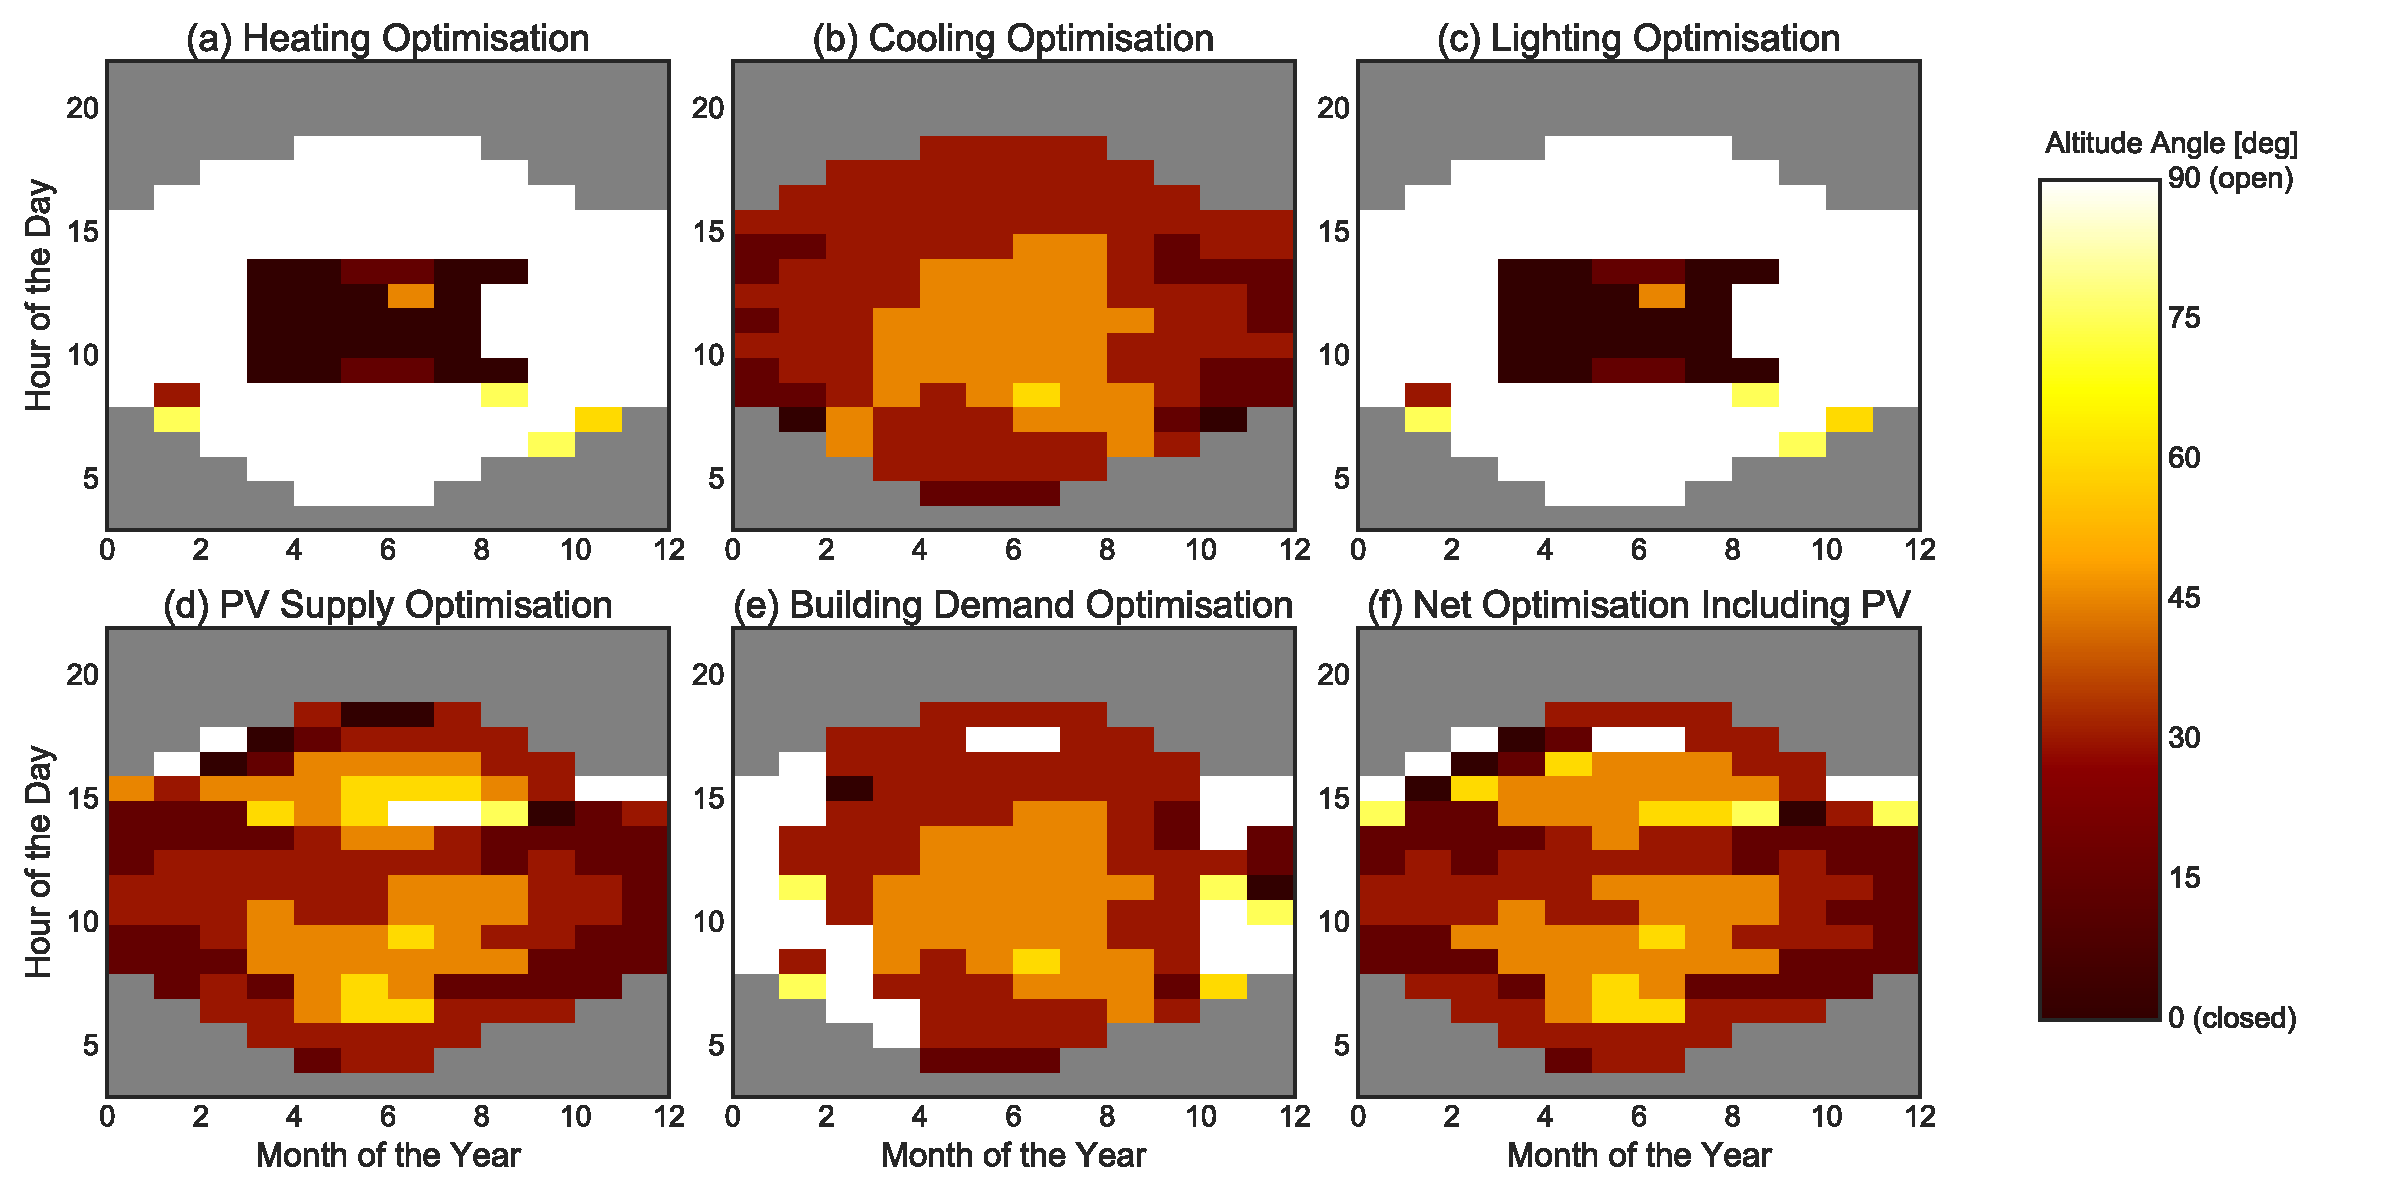
\includegraphics[width=\textwidth, trim= 0cm 0cm 0cm 0cm,clip]{Altitude.pdf}
\caption{Carpet plots detailing the optimal altitude angles to minimise the heating demand(a), cooling demand (b), lighting demand (c), and maximise PV electricity production (d). (e) details the combinations for optimum building thermal management without PV production, (f) also includes the PV production. Small angles correspond to closed positions, whereas large angles represent open positions. The corresponding azimuth angles for each hour are shown in Figure \ref{fig:monthly_azimuth}.}
\label{fig:monthly_altitude}
\end{center}
\end{figure*}

\begin{figure*}
\begin{center}
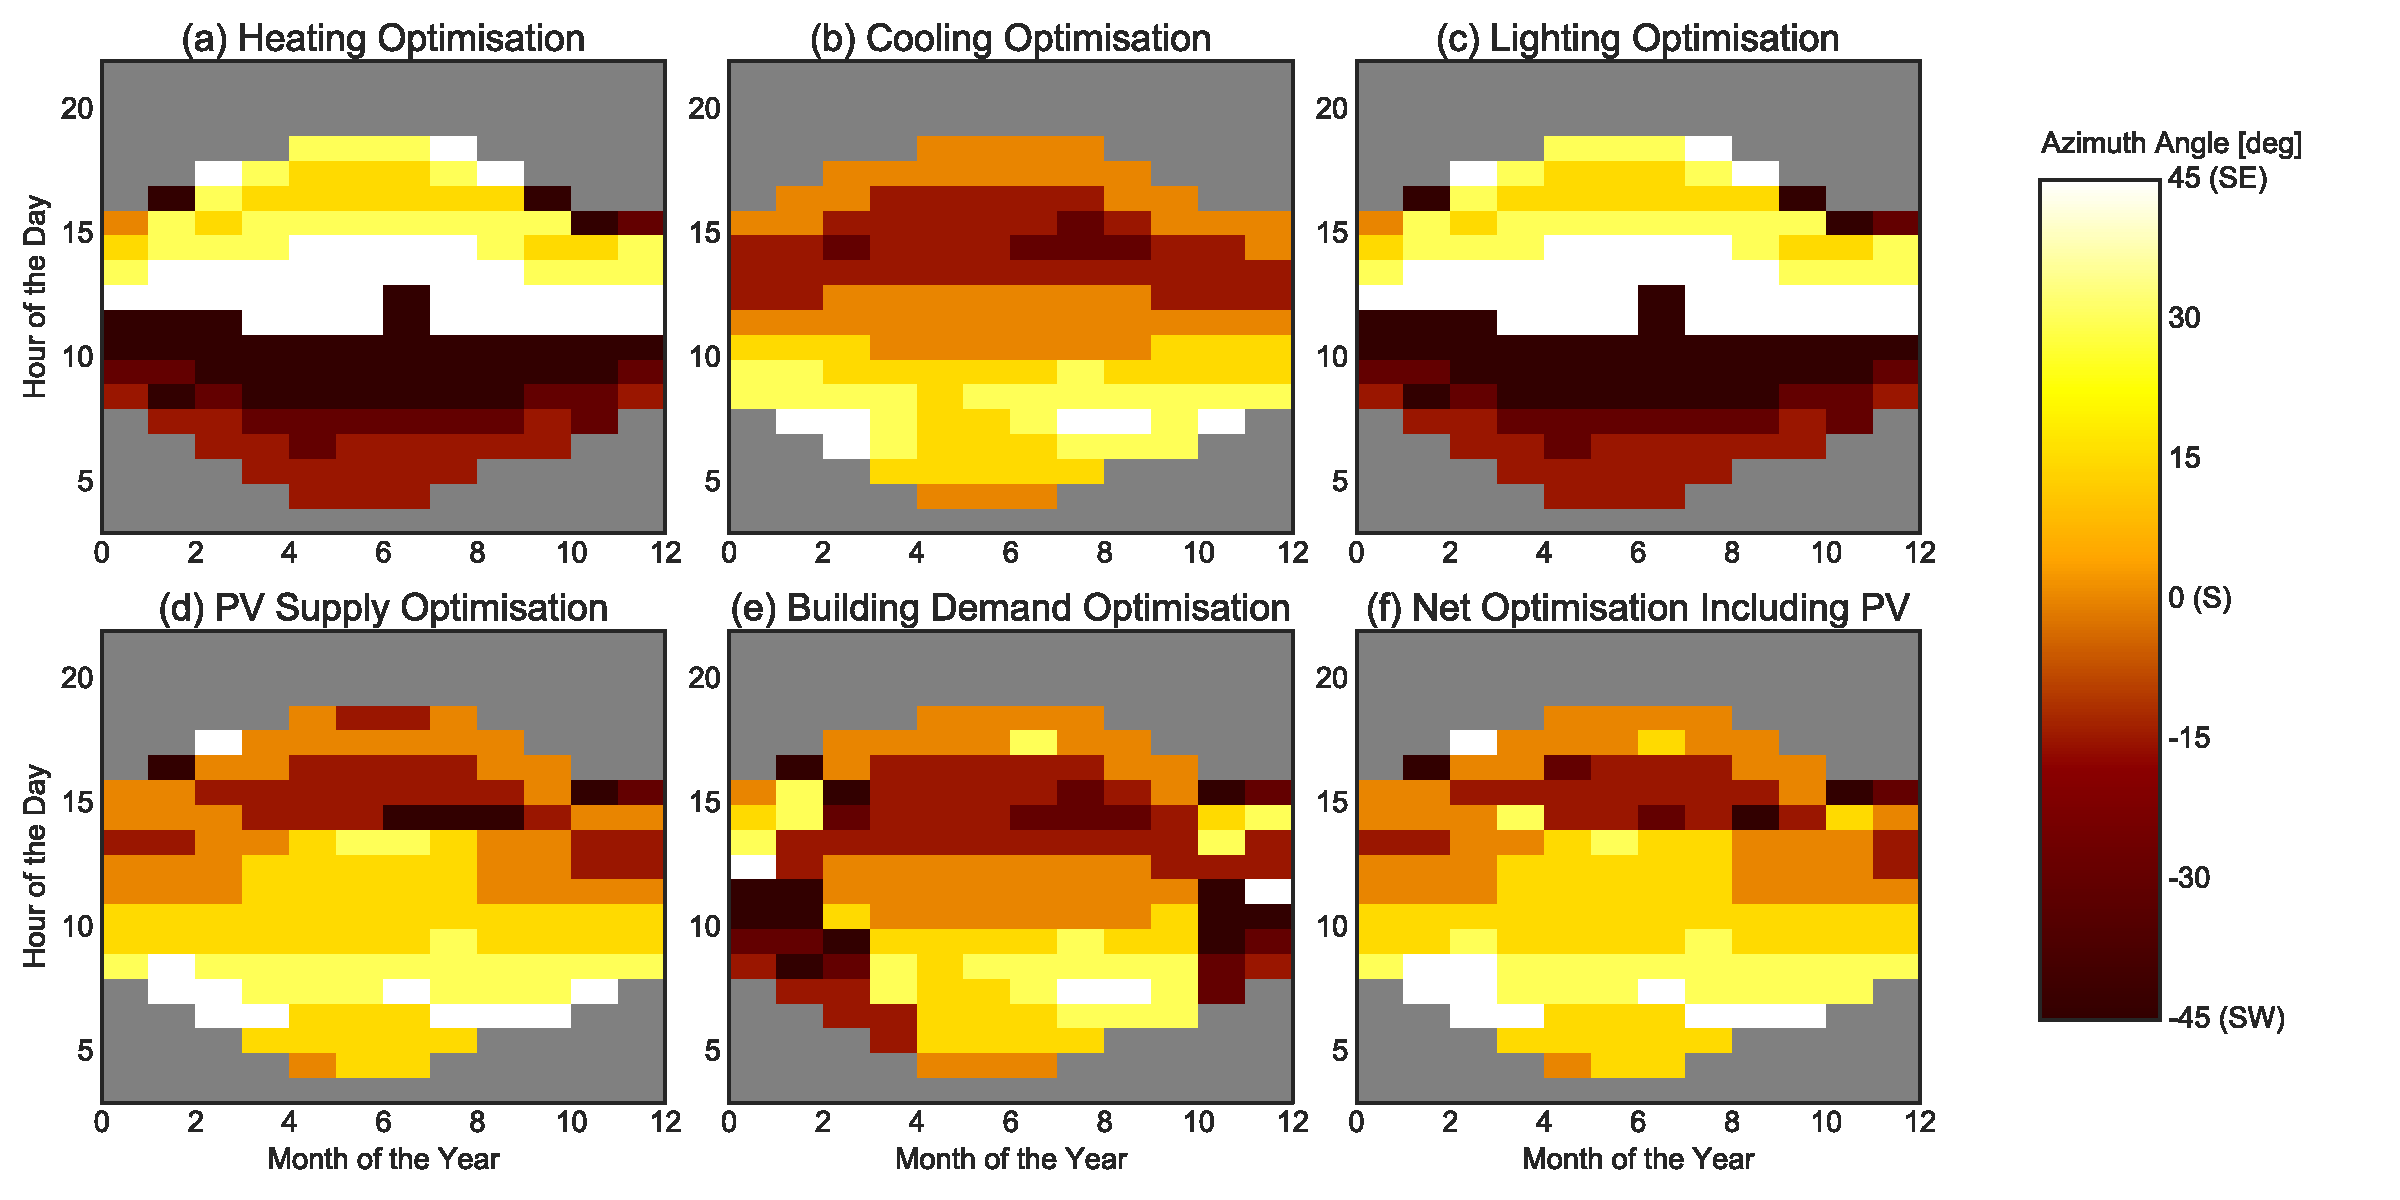
\includegraphics[width=\textwidth, trim= 0cm 0cm 0cm 0cm,clip]{Azimuth.pdf}
\caption{Carpet plots detailing the optimal azimuth angles to minimise the heating demand (a), cooling demand (b), lighting demand (c), and maximise PV electricity production (d). (e) details the combinations for optimum building thermal management without PV production, (f) also includes the PV production. Negative angles correspond to the panels facing west, whereas positive angles represent east-facing panels. The corresponding altitude angles for each hour are shown in Figure \ref{fig:monthly_altitude}.}
\label{fig:monthly_azimuth}
\end{center}
\end{figure*}



%When the four optimisation cases are combined to achieve the configurations for total energy minimisation we get some interesting results seen in Figure \ref{fig:monthly_altitude}(e) and \ref{fig:monthly_azimuth}(e). We can see that during the twilight hours of the morning and evening the open positions are preferred to minimise the use of artificial lighting. During the summer afternoons, closed positions to minimise cooling demands are preferred, however enough light is allowed to pass to sufficiently illuminate the space. When we also include the PV electricty optimisation we notice a strong tendency of the ASF to follow an optimal PV production pattern. This, however changes if the building system becomes more inefficient. Less efficient heating, for example, would result in configurations optimised for heating overpowering those of PV electricity generation.

When the four optimisation cases are combined to achieve the configurations for total energy minimisation we get interesting results, as seen in Figure \ref{fig:monthly_altitude}f and \ref{fig:monthly_azimuth}f. We see a clear tendency of the ASF to follow an optimal PV production pattern with the exception of the mid-winter evenings where heating and lighting are important. This means that it is energetically favourable to heat the room through solar radiation heat gains rather than converting the solar radiation into electricity which is then used for room heating. Configurations to reduce cooling demand are complimentary with the PV supply optimisation and therefore have a minor influence on the system control. 
%Note that these patterns were generated for a specific case study highlighted in Table \ref{tab:AssumptionsOpp}. Having a more inefficient building system may favour configurations to reduce the building energy demand over PV generation.\\


%\subsection{Net Energy Consumption}

Figure \ref{fig:carpetplot_energy} shows the net electricity use. Red colours detail the electrical consumption intensity, and blue colours detail the PV electricity surplus. It is interesting to see in Figure \ref{fig:carpetplot_energy}f how the combination of electricity generation and adaptive shading can compensate for the energy consumption of the building during most sunlit hours. Overall the PV electricity compensates for 61\% of the energy demand of the office behind the facade during the course of the year in the net energy optimisation case.

\begin{figure*}
\begin{center}
\includegraphics[width=\textwidth, trim= 0cm 0cm 0cm 0cm,clip]{carpetplot_energy3.pdf}
\caption{Carpet plots detailing the net energy consumption. Each square represents the total energy consumption for that specific hour of the entire month. Red colours detail net energy consumption, while blue colours detail net energy production.}
\label{fig:carpetplot_energy}
\end{center}
\end{figure*}


\subsection{Comparison With Other Systems}
\label{ch:comparison}

%\deleted[id=pj2]{Figure \ref{fig:compare} shows the difference between a glazing with no shading system, a static shading system, and an adaptive shading system. A south facing facade with standard glazing and no shading system would always have an overheating issue which can be seen with the large cooling load. Note that in the model there is no restriction of the heating or cooling system. This means that the cooling or heating is assumed to always meet the demand. The optimum orientation of static panels was calculated using the same simulation framework, and an orientation of 45$^{\circ}$ to the horizontal axis is a configuration close to the energy optimal state. By enabling adaptability we see how the heating load can be reduced, without compromising the cooling savings through shading. Overall, the adaptive system has a 20\% savings in the building energy demand, and a 7\% increase in PV electricity production over the static variant. }

Figure \ref{fig:compare} shows the difference between a window with no shading system, a static shading system, and an adaptive shading system which minimised net energy demand, for various coefficients of performance of the heating and cooling system. The optimum orientation of the static shading system was calculated using the same simulation framework, and a panel inclination of 45$^{\circ}$ in the altitude direction is close to the energy optimal state.

Figure \ref{fig:COP11} details an example of an inefficient building system with resistive electrical heating and a low efficiency cooling heat pump. We can see how having a simple static shading system can have a large reduction in the cooling demand with an increase in the heating demand. By including adaptability the same reduction in cooling is possible with a reduced increase in the heating demand. This effect becomes more pronounced in Figure \ref{fig:COP13} where a standard heat pump is added for cooling. Here the comparison between a static shading system and no shading is similar to the results obtained by Palmero-Marrero et al. where the reduction in the cooling demand is offset by the increase in heating demand \cite{palmero2010effect}. An adaptive facade is able to negate this loss resulting in a 44\% net energy saving compared to a building with a static facade. When an efficient heat pump heating system is also included, as detailed in Figure \ref{fig:COP33}, there is an increase in PV electricity supply by 19\%, but a negligible change in the building energy demand. This is because the angles that maximise photovoltaic generation are preferred over angles that reduce the heating demand as there is a larger net energy saving. The same results apply to a highly efficient building case as detailed in Figure \ref{fig:COP66}. Interestingly in this case, the PV supply of the ASF can almost compensate for the entire energy demand of the office space behind it. The results are summarised in Table \ref{tab:compare}.


\begin{figure}
    \centering
    \begin{subfigure}[b]{0.47\textwidth}
        \includegraphics[width=\textwidth]{compare_facadesCOP1.pdf}
        \caption{$COP_{heating}=1$, $COP_{cooling}=1$} 
        \label{fig:COP11}
    \end{subfigure} \hfill
    \begin{subfigure}[b]{0.47\textwidth}
        \includegraphics[width=\textwidth]{compare_facadesCOP1_3.pdf}
        \caption{$COP_{heating}=1$, $COP_{cooling}=3$}
        \label{fig:COP13}
    \end{subfigure}
    \vspace{10mm}

    \begin{subfigure}[b]{0.47\textwidth}
        \includegraphics[width=\textwidth]{compare_facadesCOP3.pdf}
        \caption{$COP_{heating}=3$, $COP_{cooling}=3$}
        \label{fig:COP33}
    \end{subfigure}
    \hfill
    \begin{subfigure}[b]{0.47\textwidth}
        \includegraphics[width=\textwidth]{compare_facadesCOP6.pdf}
        \caption{$COP_{heating}=6$, $COP_{cooling}=6$}
        \label{fig:COP66}
    \end{subfigure}
    \caption{Breakdown of the operational electricity consumption with no shading, with static panels at 45$^{\circ}$, and an ASF for different coefficients of performance of the heating and cooling system. (a) represents an inefficient heating and cooling system, (b) represents a standard cooling system with resistive heating, (c) represents a standard heat pump system for heating and cooling, and (d) represents a high efficiency heating and cooling system.}
    \label{fig:compare}
\end{figure}

\begin{table}
\centering

\begin{tabular}{cc|cc}


$COP_{heating}$ & $COP_{cooling}$ & ASF vs No Shading & ASF vs Static  \\
                &                 & ($$kWh/year$$)    & ($$kWh/year$$) \\
\hline 
1               & 1               & 3750  (70\%)     & 724  (31\%)   \\
1               & 3               & 1370  (62\%)      & 670  (44\%)    \\
3               & 3               & 1560  (76\%)      & 120  (20\%)    \\
6               & 6               & 1190  (97\%)      & 145  (80\%)    \\

\end{tabular}
\caption{Net electricity savings of the ASF to a building with no shading, and a static photovoltaic shading system in kWh/year.}
\label{tab:compare}
\end{table}





\section{Discussion}
\label{ch:discussion2}
\input{chapters/ch2asfSimulation/B5_discussion}

\section{Conclusion}
\label{ch:conclusion2}
% !TEX root = B99_main.tex

In this paper, we have presented a framework to model the energy performance of an adaptive photovoltaic envelope. This is achieved through the use of Radiance for the radiation simulations, an electrical circuit simulation for the PV production taking into account effects of self-shading, and a resistor-capacitor model for the building simulation. An exhaustive search optimisation algorithm computes the most energy efficient system configuration for control by minimising the heating, cooling and lighting load, while simultaneously maximising the PV electricity generation. This framework can be applied to evaluate different PV system geometries, building systems, building typologies and climates.

Our evaluation of the Adaptive Solar Facade details the advantages of the adaptive system to a static system. The ASF is able to orientate itself to the most energy efficient position, thus finding the optimum balance between PV generation, and daylight control to minimise heating, cooling and lighting demands. When optimising for heating and lighting minimisation the ASF orients to open altitude positions at 90$^{\circ}$ to the vertical plane. When optimising for PV and cooling, the ASF selects closed position, between 15$^{\circ}$ - 45$^{\circ}$ to the vertical plane. When combining all objectives for net energy minimisation there is a tendency for the ASF to follow an optimal PV production pattern with the exception of winter evenings where it is more favourable to utilise the solar heat gains for space heating and lighting. This result however, is only restricted to this case study. A less efficient heating system, for example, will result in the ASF existing in more open configurations to utilise the solar heat gains.


Our results report a 20\% - 80\% net energy saving compared to an equivalent static PV shading system depending on the efficiency of the building system. On a typical sunny winters day, the PV generation of the ASF can compensate for 62\% of the energy demand, whereas on a sunny summers day, this rises to 270\%. Over the course of the year, including cloudy days, the PV supply compensates for 61\% of the annual energy demand. This can reach 95\% in the case of a very efficient heating and cooling system with an average COP of six.

This work ultimately presents a framework for the planning and optimisation of sophisticated adaptive BIPV systems. Next stages of the research involve the utilisation of this model in our physical prototypes. The main difference in the physical model is the use of sensor data for the temperature and radiation values, as opposed to using a historical weather file. Furthermore, measuring the indoor temperature, PV electricity production, and lighting quality will create a closed loop feedback for model calibration and machine learning. 


%\added[id=pj]{Another limitation is the absence of user control. In reality, the user has the ability to override the system by opening or closing the facade to suit their desires. This override has not been included in this model, and will be evaluated through measurements of our constructed prototypes. }

%. The computation of a single configuration takes 25 seconds on a 3.4GHz processor with 16GB memory. Therefore the computation of 49 configurations assessed in this case study takes approximately 20 minutes.  A faster radiation model, or an alternative control strategy will be required to asses more configurations.




% The existing ASF prototype gives the occupant the ability to manually override the control system to open or close the ASF. 

% This occupant override has not been modelled in the case study evaluation and will reduce the overall energy saving. This will be conducted in our test environment 


%The energy saving potential and optimum orientation is also strongly dependant on the building system and weather. Decreasing the efficiency of the heating, cooling or lighting systems will give higher preference for configurations optimised for building thermal management through adaptive shading than for PV electricity production. \added[id=pj]{It is therefore important to run this framework for each individual building project to evaluate the cost-benefit ratio. }

%The optimum orientation and energy saving potential strongly depend on the geometry of the adaptive photovoltaic envelope and the efficiency of the building system. Decreasing the efficiency of the heating, cooling or lighting systems will give higher preference for configurations optimised for building thermal management through adaptive shading than for PV electricity production. 




%The algorithm compensates for this by finding configurations that minimise module self-shading. As a result, the optimum configurations for maximising PV electricity does not follow a classical solar tracking model as this would maximises self-shading, resulting in a system with lower PV generation. These losses could be minimised in the design stage by increasing the spacing between PV modules.




% In this paper, we present a simulation methodology to evaluate a dynamic photovoltaic shading system, combining both electricity generation, and the energy demand of the building. It is then coupled with a post processing python script to determine the optimum system configuration for control. The methodology can be applied to evaluate different PV system geometries, building systems, building typologies and climates.

% The dynamic PV integrated shading system has clear advantages to a static system as it can adapt itself to the external environmental conditions. This enables it to orientate itself to the most energy efficient position. The optimum orientation however, strongly depends on the general efficiency of the building. Decreasing the efficiency of the heating, cooling or lighting systems will give higher preference for configurations optimised for building thermal management through adaptive shading, than for PV electricity production.

% %The use of LED lights, for example, reduces the weighting of the lighting energy demand. This would result in closed configurations optimised for cooling to over-ride the open positions. 

% This work ultimately presents a methodology for the planning and optimisation of sophisticated adaptive BIPV systems. We are currently working on integrating the effects of module shading on PV efficiency, and the energy demand for the dynamic actuation. Future work will use this methodology to determine the environments and building typologies that could benefit from adaptive BIPV systems. 

% %Moved to Introduction: The work presented in this paper is applied in the context of the Adaptive Solar Façade (ASF) project. The ASF is a lightweight PV shading system that can be easily installed on any surface of new or existing buildings. The ASF consists of a modular frame and pneumatically actuated panels to control glare and solar gain, as well as for two-axis PV tracking. It has been implemented at the ETH House of Natural Resources will be installed at the NEST HiLo building at EMPA (www.hilo.arch.ethz.ch). 


% \section{Acknowledgments}
% \label{ch:acknowledgments}
% \input{chapters/ch2asfSimulation/7_acknowledgments}

% \begin{appendices}
%  \label{ch:appendix}
%  % !TEX root = 99_main.tex
\section{Full Set of Equations to the Building Model}

The following equations are based on the ISO 13790 standard \cite{de2008iso}. Denoting by $T_m$, the temperature of the thermal mass in the room,

\begin{equation} 
\label{eq:derrive2}
      T_m(H_{tr3}+H_{em}) + C_m {\frac{dT_m}{dt}} = \phi_{mtot}
\end{equation}

where the value $\phi_{mtot}$ represents an equivalent thermal heat flux and is given by,

\begin{equation} 
\label{eq:heatflow2}
      \phi_{mtot}= \phi_m + H_{em}T_e + \frac{H_{tr3}}{H_{tr2}}(\phi_{st} + H_wT_e + H_{tr1}T_{sup} + \frac{H_{tr1}}{H_{ve}}(\phi_{HC} + \phi_{io}))
\end{equation}

where $C_m$ is the thermal capacitance of the room, $T_e$ is the external air temperature, $T_{sup}$ is the conditioned air supply temperature. The solar heat gains $\phi_{sol}$, and internal heat gains $\phi_{int}$ are represented by three equivalent heat fluxes $\phi_{io}$, $\phi_{st}$ and $\phi_m$ which correspond to a heat exchange to the air $T_{air}$, internal room surface $T_s$, and thermal mass $T_m$ respectively. The heating and cooling heat flux is represented by $\phi_{HC}$. The five thermal conductances $H$ are represented by three equivalent conductances

\begin{equation} 
\label{eq:Htr12}
      H_{tr1}= \frac{1}{1/H_{ve} + 1/H_{is}}
\end{equation}

\begin{equation} 
\label{eq:Htr2}
      H_{tr2}= H_{tr1} + H_{w}
\end{equation}

\begin{equation} 
\label{eq:Htr32}
      H_{tr3}= \frac{1}{1/H_{tr2} + 1/H_{ms}}
\end{equation}

The internal heat flow rates due to internal gains and solar sources are divided between the thermal nodes by

\begin{equation} 
\label{eq:phi_ia2}
      \phi_{io}= 0.5\phi_{int}
\end{equation}

\begin{equation} 
\label{eq:phi_m2}
      \phi_{m}= \frac{A_m}{A_t}(0.5\phi_{int} + \phi_{sol})
\end{equation}

\begin{equation} 
\label{eq:phi_st2}
      \phi_{st}= (1-\frac{A_m}{A_t}-\frac{H_w}{9.1*A_t})(0.5\phi_{int}+\phi_{sol})
\end{equation}




Applying the Crank-Nicolson method \cite{crank1947practical} to Equation \ref{eq:derrive} gives us the discrete differential equation: 

\begin{equation} 
\label{eq:derivation2}
      T_{m_{k+1}}={\frac{\phi_{mtot}+T_{m_k}(\frac{C_m}{\Delta t} - 0.5(H_{tr3}+H_{em}))}{\frac{C_m}{\Delta t} + 0.5(H_{tr3}+H_{em})}}
\end{equation}
%  \end{appendices}



% \dictum[James C. Maxwell]{%
%   The true logic of this world is in the calculus of probabilities. }%
% \vskip 1em

% \Citet{Maxwell1865} derived some very useful equations for electromagnetic
% fields:
% \begin{align}
%     \nabla \cdot \vec{D} = \rho \\
%     \nabla \cdot \vec{B} = 0 \\
%     \nabla \times \vec{E} = -\frac{\partial \vec{B}}{\partial t} \\
%     \nabla \times \vec{H} = \vec{j} + \frac{\partial \vec{D}}{\partial t}
% \end{align}

% The energy--momentum relation, \cref{eq:energy-momentum}, is one of \emph{my}
% important results:
% \begin{align}
%     E^2 = m^2 c^4 + (p c)^2 \label{eq:energy-momentum}
% \end{align}

% Write units like this: \u{5}{\micro\meter}.

% \begin{figure}
%   \caption{A lovely face.}
% \label{fig:some-figure}
% \includegraphics{\dir/figure.pdf}
% \end{figure}
